\section{The Mamba-2 Architecture}
\label{sec:architecture}

By connecting SSMs and attention, the SSD framework allows us to develop a shared vocabulary and library of techniques for both.
In this section we discuss some examples of understanding and modifying SSD layers using ideas originally developed for Transformers.
We discuss several design choices, resulting in the Mamba-2 architecture.
These axes of variation are ablated in \cref{sec:experiments:ablations}.


\begin{figure}[!t]
  \centering
  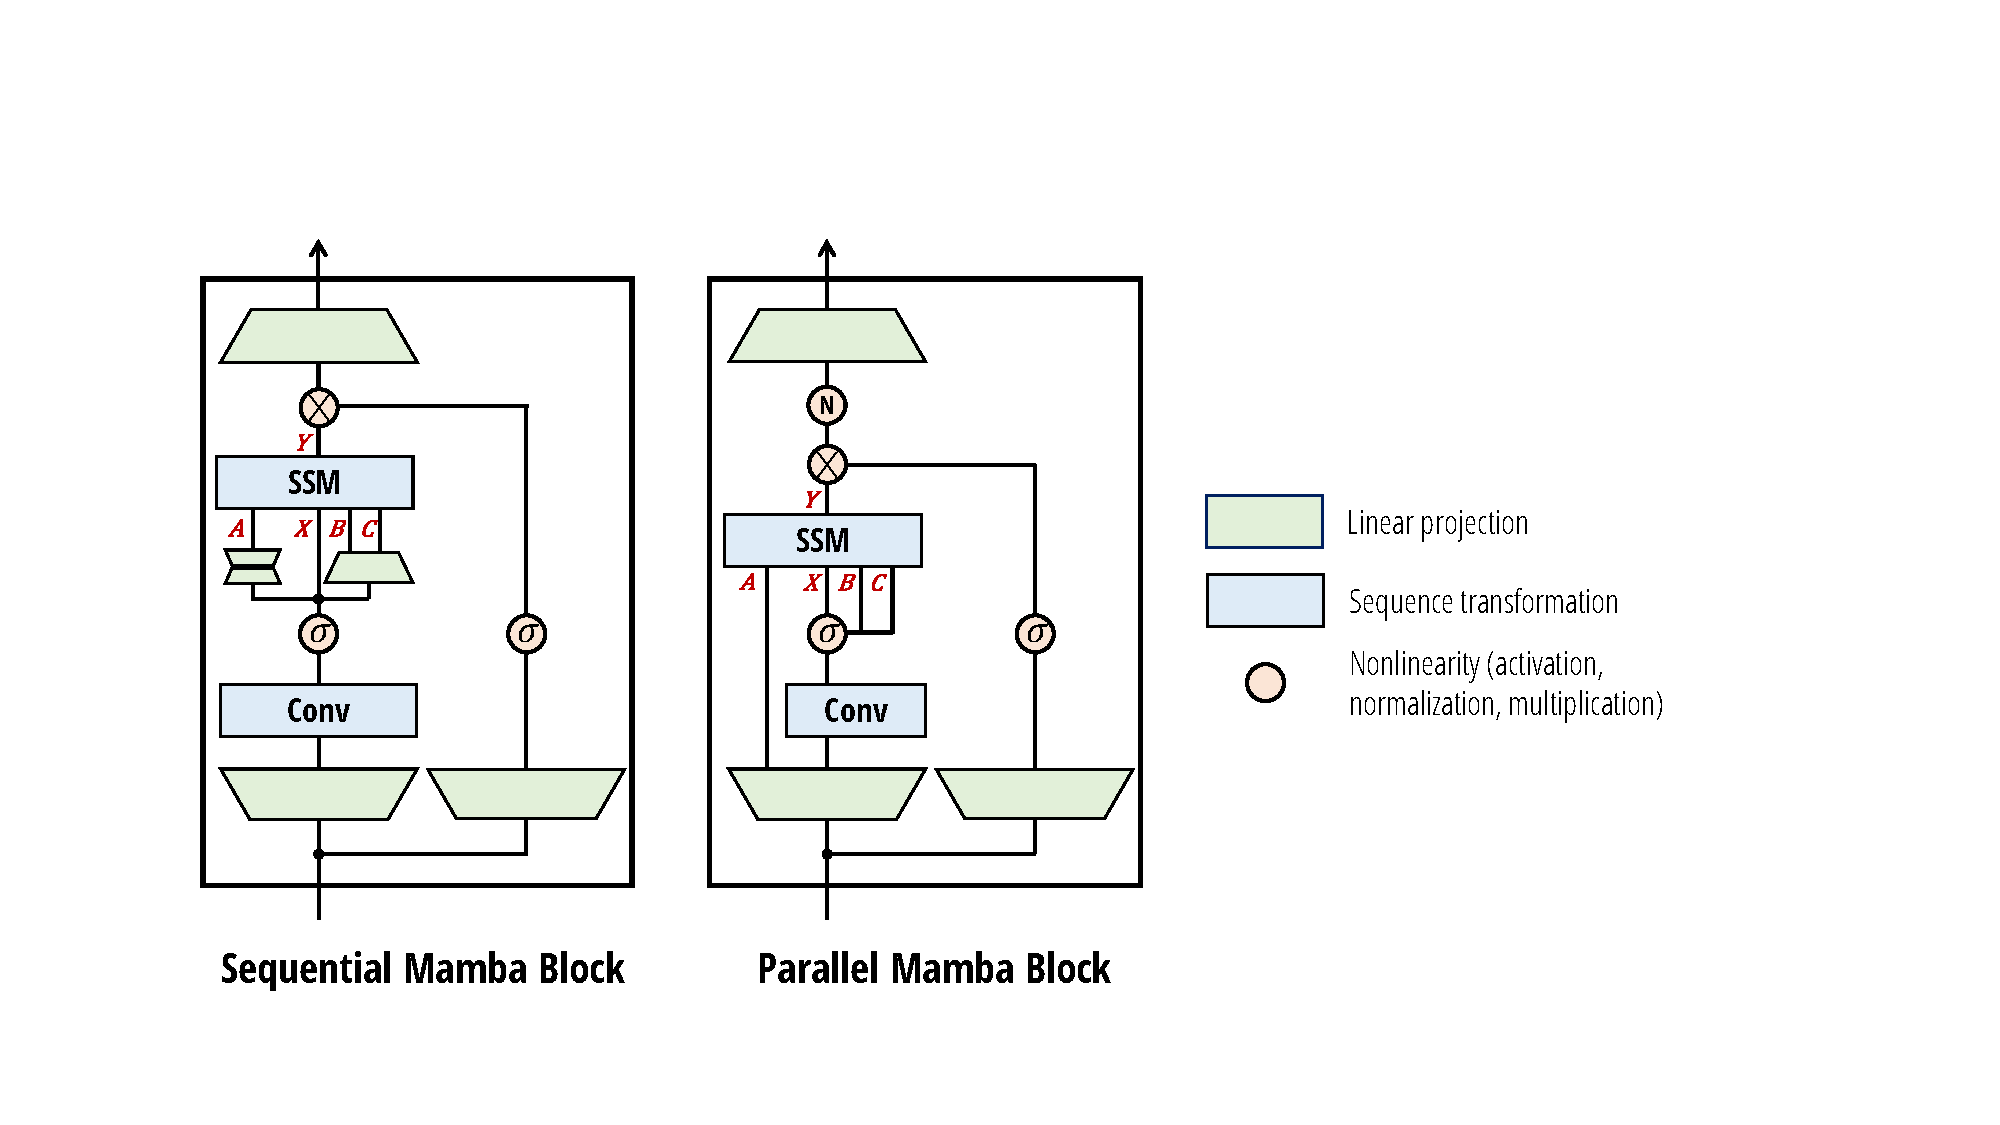
\includegraphics[width=\iftoggle{arxiv}{0.8\linewidth}{\linewidth}]{fig/architecture_2.pdf}
  \caption{
    (\textbf{Mamba-2 Architecture}.) The Mamba-2 block simplifies the Mamba block by removing sequential linear projections; the SSM parameters $A, B, C$ are produced at the beginning of the block instead of as a function of the SSM input $X$.
    An additional normalization layer is added as in NormFormer~\citep{shleifer2021normformer}, improving stability.
    The $B$ and $C$ projections only have a single head shared across the $X$ heads, analogous to multi-value attention (MVA).
  }
  \label{fig:architecture}
  \iftoggle{arxiv}{}{\vspace{-1.25em}}
\end{figure}

\subsection{Block Design}
\label{sec:architecture:block}


We first discuss modifications to the neural network block that are independent of the inner sequence mixing layer (i.e. outside the core SSD layer).

\paragraph{Parallel Parameter Projections.}

Mamba-1 was motivated by an SSM-centric point of view
where the selective SSM layer is viewed as a map from $X \mapsto Y$.
The SSM parameters $A, B, C$ are viewed as
subsidiary and are functions of the SSM input $X$.
Thus the linear projections defining $(A, B, C)$ occur after the initial linear projection to create $X$.

In Mamba-2, the SSD layer is viewed as a map from $A, X, B, C \mapsto Y$.
It therefore makes sense to produce $A, X, B, C$ in parallel with a single projection at the beginning of the block.
Note the analogy to standard attention architectures,
where $X, B, C$ correspond to the $Q, K, V$ projections that are created in parallel.

Note that adopting parallel projections for the $A, B, C, X$ inputs to the SSM slightly reduces parameters and more importantly is more amenable to tensor parallelism for larger models, by using standard Megatron sharding patterns~\citep{shoeybi2019megatron}).


\paragraph{Extra Normalization.}

In preliminary experiments, we found that instabilities were prone to arising in larger models.
We were able to alleviate this by adding an extra normalization layer (e.g. LayerNorm, GroupNorm, or RMSNorm) to the block right before the final output projection.
This usage of a normalization is most directly related to the NormFormer architecture~\citep{shleifer2021normformer}, which also added normalization layers at the end of the MLP and MHA blocks.

We also note that this change is similar to other recent models related to Mamba-2 that were derived from a linear attention viewpoint.
The original linear attention formulation normalizes by a denominator term that emulates the normalization of the softmax function in standard attention.
TransNormerLLM~\citep{qin2023transnormerllm} and RetNet~\citep{sun2023retentive} find that this normalization is unstable and add an extra LayerNorm or GroupNorm after the linear attention layer.
Our extra normalization layer differs slightly from these, occuring after the multiplicative gate branch instead of before.


\subsection{Multihead Patterns for Sequence Transformations}
\label{sec:architecture:multihead}

Recall that SSMs are defined as a sequence transformation (\cref{def:sequence-transformation})
where:
\begin{itemize}
  \item $A, B, C$ parameters have a state dimension $\mathtt{N}$.
  \item They define a sequence transformation $\R^\mathtt{T} \to \R^\mathtt{T}$, which for example can be represented as a matrix $M \in \R^{\mathtt{(T, T)}}$.
  \item This transformation operates over an input sequence $X \in \R^{\mathtt{(T, P)}}$, independently over the $\mathtt{P}$ axis.
\end{itemize}
One can view this as defining one \emph{head} of the sequence transformation.
\begin{definition}[Multihead patterns]
  \label{def:head-pattern}
  A multihead sequence transformation consists of $\mathtt{H}$ independent heads, for a total model dimension of $\mathtt{D}=\mathtt{d\_model}$.
  The parameters may be tied across heads, leading to a \textbf{head pattern}.
\end{definition}
The state size $\mathtt{N}$ and head dimension $\mathtt{P}$ are analogous to the $QK$ head dimension and $V$ head dimension of attention, respectively.
Just as in modern Transformer architectures~\citep{chowdhery2022palm,touvron2023llama},
in Mamba-2 we generally choose these to be constants around $64$ or $128$; when the model dimension $\mathtt{D}$ increases, we increase the number of heads while keeping the head dimensions $\mathtt{N}$ and $\mathtt{P}$ fixed.
In order to describe how to do this,
we can transfer and generalize ideas from multihead attention to define similar patterns for SSMs, or any general sequence transformation.

\begin{minipage}[t]{.25\linewidth}
  \begin{equation}%
    \label{eq:multihead}
    \begin{aligned}%
        & \textbf{Multi-head SSM} \\
        & (\textrm{Multi-head Attn.}) \\
      X & \quad \mathtt{(T, H, P)} \\
      A & \quad \mathtt{(T, H)} \\
      B & \quad \mathtt{(T, H, N)} \\
      C & \quad \mathtt{(T, H, N)} \\
    \end{aligned}
  \end{equation}
\end{minipage}
\begin{minipage}[t]{.25\linewidth}
  \begin{equation}%
    \label{eq:multiquery}
    \begin{aligned}%
    & \textbf{Multi-contract SSM} \\
    & (\textrm{Multi-query Attn.}) \\
      X & \quad \mathtt{(T, 1, P)} \\
      A & \quad \mathtt{(T, H)} \\
      B & \quad \mathtt{(T, 1, N)} \\
      C & \quad \mathtt{(T, H, N)} \\
    \end{aligned}
  \end{equation}
\end{minipage}
\begin{minipage}[t]{.25\linewidth}
  \begin{equation}%
    \label{eq:multikey}
    \begin{aligned}%
    & \textbf{Multi-expand SSM} \\
    & (\textrm{Multi-key Attn.}) \\
      X & \quad \mathtt{(T, 1, P)} \\
      A & \quad \mathtt{(T, H)} \\
      B & \quad \mathtt{(T, H, N)} \\
      C & \quad \mathtt{(T, 1, N)} \\
    \end{aligned}
  \end{equation}
\end{minipage}
\begin{minipage}[t]{.25\linewidth}
  \begin{equation}%
    \label{eq:multivalue}
    \begin{aligned}%
    & \textbf{Multi-input SSM} \\
    & (\textrm{Multi-value Attn.}) \\
      X & \quad \mathtt{(T, H, P)} \\
      A & \quad \mathtt{(T, H)} \\
      B & \quad \mathtt{(T, 1, N)} \\
      C & \quad \mathtt{(T, 1, N)} \\
    \end{aligned}
  \end{equation}
\end{minipage}

\paragraph{Multihead SSM (MHS) / Multihead Attention (MHA) Pattern.}

The classic MHA pattern assumes that the head dimension $\mathtt{P}$ divides the model dimension $\mathtt{D}$.
The number of heads is defined as $\mathtt{H} = \mathtt{D} / \mathtt{P}$.
Then, $\mathtt{H}$ copies of the core sequence transformation are created by creating $\mathtt{H}$ independent copies of each parameter.
Note that while the MHA pattern was first described for the attention sequence transformation,
it can be applied to anything compatible with \cref{def:sequence-transformation}.
For example, a multi-head SSD layer would accept inputs with shapes according to equation \eqref{eq:multihead}
where the SSD algorithm is broadcasted over the $\mathtt{H} = \mathtt{n\_heads}$ dimension.

%

\paragraph{Multi-contract SSM (MCS) / Multi-query Attention (MQA) Pattern.}

Multi-query attention~\citep{shazeer2019fast} is a clever optimization for attention that can dramatically improve the speed of autoregressive inference,
which relies on caching the $K$ and $V$ tensors.
This technique simply avoids giving $K$ and $V$ the extra head dimension,
or in other words broadcasts a single head of $(K, V)$ across all the heads of $Q$.

Using the state space duality, we can define an equivalent SSM version of MQA as equation \eqref{eq:multiquery}.
Here, $X$ and $B$ (the SSM analogs of attention's $V$ and $K$) are shared across the $\mathtt{H}$ heads.
We also call this the \emph{multi-contract SSM (MCS)} head pattern, because the $C$ parameter which controls the SSM state contraction has independent copies per head.

We can similarly define a multi-key attention (MKA) or \emph{multi-expand SSM (MES)} head pattern,
where $B$ (which controls the SSM expansion) is independent per head while $C$ and $X$ are shared across heads.

\paragraph{Multi-input SSM (MIS) / Multi-value Attention (MVA) Pattern.}

While MQA makes sense for attention because of its KV cache, it is not the natural choice for SSMs.
In Mamba, instead, $X$ is viewed as the main input to the SSM,
and therefore $B$ and $C$ are parameters that are shared across the input channels.
We define a new multi-value attention (MVA) of \emph{multi-input SSM (MIS)} pattern in equation \eqref{eq:multivalue}, which can again be applied to any sequence transformation such as SSD.

Armed with this vocabulary, we can characterize the original Mamba architecture more precisely.
\begin{proposition}
  \label{prop:mamba-multihead}
  The selective SSM (S6) layer of the Mamba architecture~\citep{gu2023mamba} can be viewed as having
  \begin{itemize}
    \item Head dimension $P=1$: every channel has independent SSM dynamics $A$.
    \item \emph{Multi-input SSM} (MIS) or \emph{multi-value attention} (MVA) head structure: the $B, C$ matrices (corresponding to $K, Q$ in the attention duality) are shared across all channels of the input $X$ (corresponding to $V$ in attention).
  \end{itemize}
\end{proposition}

We can also ablate these head pattern variants when applied to SSD (\cref{sec:experiments:ablations:kernels}).
Interestingly, despite being controlled in parameter counts and total state dimension,
there is a noticeable difference in downstream performance.
We empirically find that the MVA pattern as originally used in Mamba performs best.

\paragraph{Grouped Head Patterns.}

The ideas of multi-query attention can be extended to \emph{grouped-query attention}~\citep{ainslie2023gqa}: instead of $1$ K and V head, one can create $\mathtt{G}$ independent K and V heads, where $1 < \mathtt{G}$ and $\mathtt{G}$ divides $\mathtt{H}$.
This is motivated both by bridging the performance difference between multi-query and multi-head attention,
and enabling more efficient tensor parallelism by setting $\mathtt{G}$ to be a multiple of the number of shards (\cref{sec:systems}).

Similarly, the multi-input SSM head pattern used in Mamba-2 can be easily extended to \textbf{grouped-input SSM (GIS)}, or synonymously \textbf{grouped-value attention (GVA)}.
The generalization is straightforward and we omit the details for simplicity.


\subsection{Other SSD Extensions from Linear Attention}
\label{sec:architecture:kernels}

We describe here an example of architectural modifications to SSD motivated by linear attention.
We ablate these in \cref{sec:experiments:ablations:kernels} as a form of negative result,
finding that they do not significantly improve performance enough to adopt them as default settings.
Nonetheless, these illustrate how the vast literature on attention can be incorporated to
define variants of SSD.
We treat the choice of kernel feature map as a hyperparameter in the Mamba-2 architecture,
and expect other simple modifications inspired by attention to be possible as well.

\paragraph{Kernel Attention Approximations to Softmax Attention.}
Many variants of linear attention or kernel attention are motivated by viewing the attention scores $\mathsf{softmax}(QK^{\top})$ as composed of
\begin{enumerate}
  \item An exponential kernel $Z = \exp(QK^{\top})$, which can be approximated by $Z = \psi(Q)\psi(K)^{\top}$ for some kernel feature map.
  \item Normalizing the kernel so that rows sum to $1$ via $M = G / G \bm{1} \bm{1}^{\top}$, where the division happens elementwise and $\bm{1}$ is the all 1's vector.
\end{enumerate}

\paragraph{Exponential Kernel Feature Maps.}

In Mamba-2, we incorporate a flexible kernel feature map, and apply it to the $B$ and $C$ branches (corresponding to the $K$ and $V$ branches in attention).
The feature map can also be optionally applied to the $X$ ($V$) branch, for simplicity and symmetry.
This is represented in \cref{fig:architecture} by an arbitrary nonlinearity.
By default, we simply choose $\psi$ to be an elementwise Swish / SiLU function~\citep{hendrycks2016gaussian,ramachandran2017swish}.
We explore other options in the ablations in \cref{sec:experiments:ablations:kernels},
including feature maps used by Linear Attention, Performer, Random Feature Attention, and cosFormer (\cref{sec:attention:kernel}).

\paragraph{Incorporating a Normalization (Denominator) Term.}

To find the denominator term, we simply have to compute $M \bm{1}$.
But recall that the final output of the model is just $Y = MX$ (equation \eqref{eq:ssm-quad}).
So the normalization terms can be found
simply by augmenting $X$ with an extra column $\bm{1}$, resulting in a tensor of shape $\mathtt{(T, P+1)}$.

Note that in this case, the kernel feature map $\psi$ must be positive so that the sum is positive.
